\documentclass{article}

% load tikz core package
\usepackage{tikz}

% load aditional tikz packages
\usetikzlibrary{arrows.meta,
    decorations.pathmorphing,
    backgrounds,
    positioning,
    fit,
    petri}

% styles
\tikzset{
  place/.style={circle, draw=blue!50, fill=blue!20, thick, minimum size=6mm, inner sep=0pt},
  transition/.style={rectangle, draw=black!50, fill=black!20, thick, minimum size=4mm, inner sep=0pt},
  }

\begin{document}
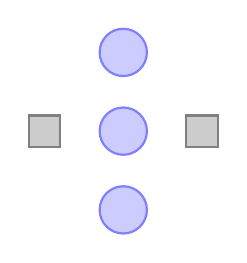
\begin{tikzpicture}
  % instead of drawing shapes, we use nodes
  \node [place]      (waiting)        at (0,2)  {};
  \node [place]      (critical)       at (0,1)  {};
  \node [place]      (semaphore)      at (0,0)  {};
  \node [transition] (leave critical) at (-1,1) {};
  \node [transition] (enter critical) at (1,1)  {};
\end{tikzpicture}
\end{document}